\chapter{Modelo de cámara}

\section{Modelo \emph{pinhole}}

Una cámara, por medio de una proyección central, establece una correspondencia entre puntos del espacio con puntos bidimensionales en su plano imágen. En particular se estudia el modelo de cámara \emph{pinhole} \cite{LibroCompGrafica3}.

Se considera el centro de proyección $C$, también centro óptico de la cámara, como el orígen de un sistema de coordenadas euclideano, y $Z = f$ el plano de la imagen o plano focal.

\begin{figure}[H]
  \centering
    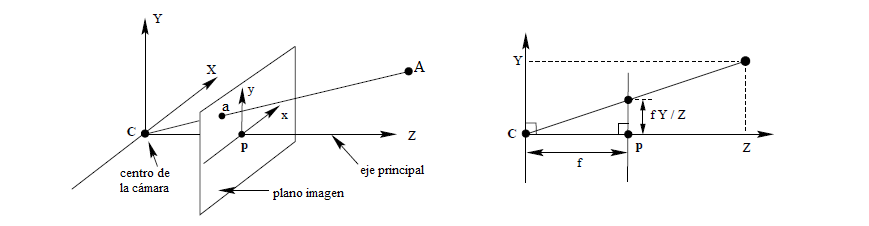
\includegraphics[width=0.8\textwidth]{./Cap2_videomapping/pinhole.png}
  \caption[Multiple View Geometry in Computer Vision, Fig. 6.1]{Geometría de cámara \emph{pinhole}. $C$ es centro de la cámara y $p$ el punto principal}
  \label{fig:Calib-Pinhole}
\end{figure}

Un punto en el espacio $A=(A_X, A_Y, A_Z)^T$ se corresponde con el punto $a$ en el plano imagen, dado por la intersección del rayo que pasa por el centro de cámara y el punto $A$ con el plano imagen. El punto $A$ se corresponde con $(\frac{fA_X}{A_Z}, \frac{fA_Y}{A_Z}, f)^T$ en el plano imagen considerando que el centro de coordenadas del plano coincide con el punto principal $P$.

Considerando la representación de los puntos como vectores homogéneos se expresa la proyección central como una correspondencia lineal entre las coordenadas homogéneas.

\[
\begin{pmatrix}
A_X \\ A_Y \\ A_Z \\ 1
\end{pmatrix}
\to
\begin{pmatrix}
fA_X \\ fA_Y \\ A_Z
\end{pmatrix}
=
\begin{pmatrix}
f & 0 & 0 & 0 \\
0 & f & 0 & 0 \\
0 & 0 & 1 & 0 \\
\end{pmatrix}
\begin{pmatrix}
A_X \\ A_Y \\ A_Z \\ 1
\end{pmatrix}
\]

Dado $A_h = (A_X,A_Y,A_Z,1)^T$ y la proyección $a$ sobre el plano imagen, la correspondencia utilizando el método pinhole es:
$a=PA_h$

Siendo
\[
P = 
\begin{pmatrix}
f & 0 & 0 & 0 \\
0 & f & 0 & 0 \\
0 & 0 & 1 & 0 \\
\end{pmatrix}
\]

\section{Geometría epipolar}
La geometría epipolar\cite{LibroCompGrafica3} es la geometría proyectiva intrínseca entre dos puntos de vista. Es dada por la intersección de los planos imagen de cada cámara con el plano epipolar. Este plano es el definido por el punto a representar $X$ y los dos centros de las cámaras $C$ y $C'$.

\begin{figure}[H]
  \centering
    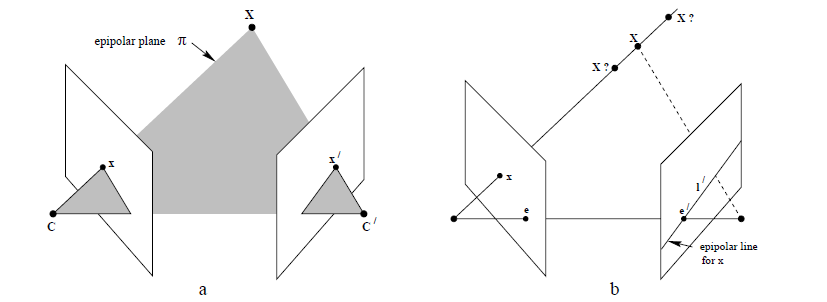
\includegraphics[width=0.7\textwidth]{./Cap2_videomapping/epipolar.PNG}
  \caption[Multiple View Geometry in Computer Vision, Fig. 9.1]{$C$ y $C'$ centos de las cámaras.}
  \label{fig:Epipolar}
\end{figure}
La matriz fundamental $F$ es la representación algebraica de la geometría epipolar.
Dado un par de imágenes, como se muestra en la figura para cada punto $x$ en una imagen existe una linea epipolar correspondiente $l'$ en la otra imagen. Cualquier punto $x'$ en la segunda imagen que corresponde al punto $x$, debe pertenecer a la linea epipolar $l'$.
La línea epipolar $l'$ es la proyección en la segunda imagen del rayo que parte del punto $x$ y llega al centro $C$ de la primer cámara. Se establece por tanto un mapeo de un punto en una imagen con la línea epipolar en la otra imagen.
\[  x \to l'
\]
 
El mapeo de puntos a líneas es representado por $F$ la matriz fundamental.

\begin{figure}[H]
  \centering
    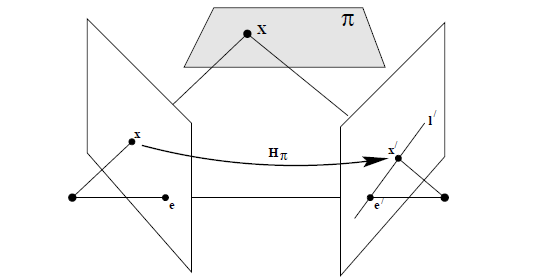
\includegraphics[width=0.7\textwidth]{./Cap2_videomapping/epipolar2.PNG}
  \caption[Multiple View Geometry in Computer Vision, Fig. 9.5]{Matriz fundamental $F$.}
  \label{fig:Epipolar2}
\end{figure}
Dado $x$ en una imagen se corresponde con el punto $x'$ en la segunda imagen vía una trasferencia establecida por la intersección del plano $\pi$ con los planos imagen de cada cámara.
La línea epipolar que contiene $x'$ se obtiene uniendo $x'$ con el epipolo $e'$, esto es:
\[ x' = H_{\pi} * x \]    siendo  $H_{\pi}$ una homografía 2D que establece la correspondencia entre cada $x_i$ de la primer imagen a $x'_i$ en la segunda imagen.
\[ l' = e' * x' = e' * H_{\pi} * x = F * x  \]
\[ F = e' * H_{\pi}  \mbox{es la matriz fundamental}  \]